\documentclass{article}

\usepackage{enumerate}
\usepackage{amsmath,amsthm,amssymb}
\usepackage{tikz}
\usepackage{pgfplots}
\usepackage{multicol}
%\pgfplotsset{compat=newest}

\usepackage[margin=1in]{geometry}

\begin{document}

\noindent \textbf{Name:}\underline{\hspace{2in}} \hfill \textbf{Quiz 2: September 6}
\vspace{1em}

\noindent Let $f$ be the \emph{greatest integer function} $f(x) = [x]$ we saw in class. Let $g$ be the function $g(x) = 1/x$, and $h$ be the absolute value function $h(x) = |x|$. As always, show your work.
\begin{enumerate}
\item The graph $y = f(x)$ is reproduced below.
  \begin{multicols}{2}
    \begin{center}
      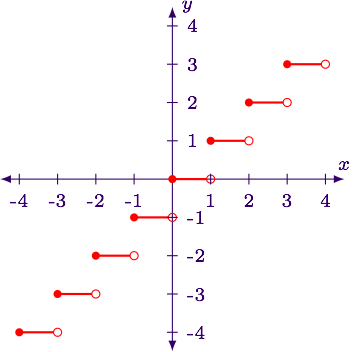
\includegraphics[width=\columnwidth]{greatest-integer.png}
    \end{center}
  \begin{enumerate}
  \item What are the $x$-intercepts of $y = f(x)$?
    \vspace{0.75in}
  \item Which of $f$, $g$, and $h$ are even functions?
    \vspace{1in}
  \item Which of $f$, $g$, and $h$ are odd functions?
  \end{enumerate}
\end{multicols}
\vspace{0.5in}
\item
  \begin{enumerate}
  \item Write an algebraic expression for $f \circ g$ and $g \circ f$.
    \vspace{0.75in}
  \item What is the domain of $g \circ f$? (Per usual, express your answer in interval notation.)
    \vspace{0.75in}
  \end{enumerate}

\item Children who grow up in houses with books typically perform well on the SAT. Take $b(x)$ to be a function whose input is ``number of books in house'' and output is ``expected SAT score.''
  \begin{enumerate}
  \item What are the two types of local extrema? (Just tell me the words from class.)
    \vspace{0.5in}
  \item  What does each type of local extremum mean, in the context of this function $b$?
  \end{enumerate}

  

\end{enumerate}

\end{document}
